\documentclass[11pt]{article}
\usepackage[utf8]{inputenc}
\usepackage[english, ngerman]{babel}
\usepackage{amsmath,amsthm,verbatim,amssymb,amsfonts,amscd}
\usepackage{enumerate}
\usepackage{listings}
\usepackage{courier}
\usepackage{graphicx}
\usepackage{epstopdf}
\usepackage[margin=1in]{geometry}
\lstset{
  numbers=left,
  language=C,
  basicstyle=\footnotesize\ttfamily,
  breaklines=true,
  morekeywords={function, NIL}
}
\newcommand{\abs}[1]{\left| #1 \right| }
\setlength{\parindent}{0pt} 

\author{
  Felix Schrader, 3053850 \\ 
  Jens Duffert, 2843110 \\
  Eduard Sauter, 3053470
}
\title{Datenstrukturen und Algorithmen: Haus\"ubung 11}
\begin{document}
\maketitle


\subsection*{Aufgabe 1}
Es soll folgende Sequenz sortiert werden: 77, 31, 23, 11, 56, 32, 75, 45
\begin{enumerate}[a)]
    \item mit Bubble Sort\\
        Ausgangssequenz:\\
        77, 31, 23, 11, 56, 32, 75, 45\\
        Nun wird Bubble Sort angewendet:\\
        31, 77, 23, 11, 56, 32, 75, 45 \\
        31, 23, 77, 11, 56, 32, 75, 45 \\
        31, 23, 11, 77, 56, 32, 75, 45 \\
        31, 23, 11, 56, 77, 32, 75, 45 \\
        31, 23, 11, 56, 32, 77, 75, 45 \\
        31, 23, 11, 56, 32, 75, 77, 45 \\
        31, 23, 11, 56, 32, 75, 45, 77 \\
        23, 31, 11, 56, 32, 75, 45, 77 \\
        23, 11, 31, 56, 32, 75, 45, 77 \\
        23, 11, 31, 32, 56, 75, 45, 77 \\
        23, 11, 31, 32, 56, 45, 75, 77 \\
        11, 23, 31, 32, 56, 45, 75, 77 \\
        11, 23, 31, 32, 45, 56, 75, 77 \\


    \item[b)]

        Die oben genannte Frequenz soll nun mit Merge Sort sortiert werden.\\
        \begin{figure}
            \centering
            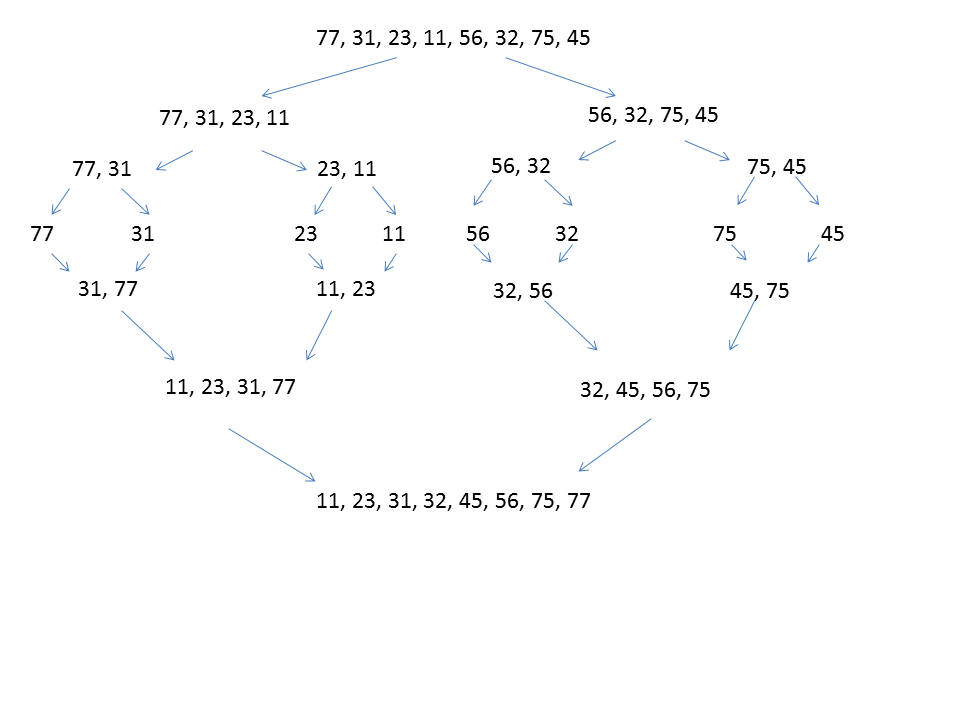
\includegraphics[width=0.7\linewidth]{aufgabeeins_b.png}

        \end{figure}


\end{enumerate}


\subsection*{Aufgabe 2}
\begin{enumerate}[a)]
  \item Implementation von \texttt{partition}
    \lstinputlisting{quicksort.js}
  \item
    \begin{itemize}
      \item Ja, das ist korrekt. Man kann den Vorgang überschlagen.
        Für den Worst-Case beschränkt man sich auf den größeren Teil des
        Arrays beschränken, der nach einer Partitionierung mit
        1000 zu 1 noch übrig bleibt. Nach $x$ Schritten muss dann
        %
        \begin{align*}
          N \left( \frac{1000}{1001} \right)^x = 1
        \end{align*}
        %
        sein.
        Also ist dann
        %
        \begin{align*}
          x = \log_{\frac{1000}{1001}} (\frac{1}{N}) =  k \log_2(N)
        \end{align*}
        %
        Mit einer negativen Konstanten $k$. Damit ist dann die Gesamtlaufzeit auch
        wieder $\mathcal{O}(N \log_2(N))$.

      \item Das ist nicht korrekt. Im schlimmsten fall kann das Array immer
        noch sortiert sein und zufällig das Element am Ende oder Anfang ausgewählt
        werden. Auch wenn dies deutlich unwahrscheinlicher ist.

      \item Ja, da Partition für ein Array der Länge $n$ $\mathcal{O}(n)$
        Zeit benötigt. Ein zusätzlicher Zeitaufwand in $\mathcal{O}(n)$ ändert
        also an der Laufzeit nichts, da immer noch nur zur Hälfte partitioniert
        wird durch das Finden eines optimalen Elementes.

      \item Ja, denn man garantiert dann eine Partitionierung in hälften.
        Da \texttt{median} in $\mathcal{O}(n)$ realisierbar ist, erhält man
        dann eine Worst-Case Laufzeit von $\mathcal{O}(n \log(N))$.

    \end{itemize}
\end{enumerate} 

\subsection*{Aufgabe 3}
  \begin{enumerate}[a)]
    \item 
      \begin{align*}
        \texttt{i=0:} & & \\
        \texttt{a} & & \\ 
        \texttt{b} & & \\ 
        \vdots & & \\ 
        \texttt{g} & \rightarrow \texttt{graph} & \\ 
        \vdots & & \\ 
        \texttt{p} & \rightarrow \texttt{position, partition, pivot, parität}
          & \rightarrow \texttt{i=1 (p)} \\ 
        \vdots & & \\ 
        \texttt{s} & \rightarrow \texttt{stack, speicher, stapelspeicher}
          & \rightarrow \texttt{i=1 (s)} \\ 
        \vdots & & \\ 
        \texttt{z} & & \\ 
        \texttt{i=1 (p):} & & \\
        \texttt{a} & \rightarrow \texttt{partition, parität} & \rightarrow
          \texttt{i=2 (pa)} \\ 
        \vdots & & \\ 
        \texttt{i} & \rightarrow \texttt{pivot} & \\ 
        \vdots & & \\ 
        \texttt{o} & \rightarrow \texttt{position} & \\ 
        \vdots & & \\ 
        \texttt{i=2 (pa):} & & \\
        \vdots & & \\ 
        \texttt{r} & \rightarrow \texttt{partition, parität} & \rightarrow
          \texttt{i=3 (par)} \\ 
        \vdots & & \\ 
      \end{align*}
      \begin{align*}
        \texttt{i=3 (par):} & & \\
        \vdots & & \\ 
        \texttt{i} & \rightarrow \texttt{parität} & \\ 
        \vdots & & \\ 
        \texttt{t} & \rightarrow \texttt{partition} & \\ 
        \vdots & & \\ 
        \texttt{i=1 (s):} & & \\ 
        \vdots & & \\ 
        \texttt{p} & \rightarrow \texttt{speicher} & \\ 
        \vdots & & \\ 
        \texttt{t} & \rightarrow \texttt{stack, stapelspeicher} & \rightarrow
          \texttt{i=2 (st)} \\ 
        \vdots & & \\ 
        \texttt{i=2 (st):} & & \\ 
        \texttt{a} & \rightarrow \texttt{stack, stapelspeicher} & \rightarrow
          \texttt{i=3 (sta)} \\ 
        \vdots & & \\ 
        \texttt{i=3 (sta):} & & \\
        \vdots & & \\ 
        \texttt{c} & \rightarrow \texttt{stack} & \\ 
        \vdots & & \\ 
        \texttt{p} & \rightarrow \texttt{stapelspeicher} & \\ 
        \vdots & & \\ 
      \end{align*}
      \texttt{Sortierung: graph, parität, partition, pivot, position, speicher,
        stack, stapelspeicher}
    \item 
      Der Algorithmus lässt sich auf Zahlen übertragen, indem man statt der
      Sortierung \texttt{a,\dots z} die Reihenfolge \texttt{0,\dots 9}
      verwendet. Allerdings muss man vorher die Zahl mit den meisten Stellen
      finden und bei kürzeren Zahlen so viele Nullen vorne hinzufügen, dass sie
      gleich lang sind (sonst wäre z.B. \texttt{9>10} möglich).
    \item 
  \end{enumerate}
\end{document}
